\documentclass[11pt,fleqn]{article}
%\usepackage{CJK}
\usepackage{latexsym}
\usepackage{color}
\usepackage{graphicx, float}\usepackage{graphicx}
%\usepackage{algorithmicx}
\usepackage{algorithm}
\usepackage{algpseudocode}
%\usepackage[colorlinks]{hyperref}
\setlength{\oddsidemargin}{-0.0in}
\setlength{\evensidemargin}{-0.0in} \setlength{\textwidth}{6.0in}
\setlength{\textheight}{9.0in} \setlength{\topmargin}{-0.2in}

%\setlength{\leftmargin}{0.7in}
\usepackage{amssymb, graphicx, amsmath}  %  fancyheadings,

\newcommand\qed{\qquad $\square$}
\newcommand{\nn}{\nonumber}

\def \[{\begin{equation}}
\def \]{\end{equation}}
\def\proof{{\bf Proof:\quad}}
\def \endzm {\quad $\Box$}
\def\dist{\hbox{dist}}


\newcommand{\R}{\mathbb{R}}
%\newtheorem{yinli}{����}[section]
\newcommand{\D}{\displaystyle}
\newcommand{\T}{\textstyle}
\newcommand{\SC}{\scriptstyle}
\newcommand{\FT}{\footnotesize}



%\newtheorem{theorem}{Theorem}[section]
%\renewcommand{\thetheorem}{\arabic{section}.\arabic{theorem}}
\newtheorem{definition}{Definition}
\renewcommand{\thedefinition}{\arabic{section}.\arabic{definition}}
\newtheorem{lemma}{Lemma}[section]
\renewcommand{\thelemma}{\arabic{section}.\arabic{lemma}}
\newtheorem{remark}{Remark}
\renewcommand{\theremark}{\arabic{section}.\arabic{remark}}
\newtheorem{proposition}{Proposition}[section]
\renewcommand{\theproposition}{\arabic{section}.\arabic{proposition}}
\newtheorem{corollary}{Corollary }[section]
\renewcommand{\thecorollary}{\arabic{section}.\arabic{corollary}}
\renewcommand{\theequation}{\arabic{section}.\arabic{equation}}
\renewcommand{\baselinestretch}{1.35}
\newtheorem{exam}{Example}[section]
\renewcommand{\theexam}{\arabic{section}.\arabic{exam}}
\newtheorem{theo}{Theorem}[section]
\renewcommand{\thetheo}{\arabic{section}.\arabic{theo}}
\begin{document}
%\begin{CJK*}{GBK}{song}

\begin{center}

{\LARGE \bf  Machine Learning and Computer Vision Assignment 4}\\


\vskip 25pt
 {Huihuang Zheng, huihuang@utexas.edu }\\
\vskip 5pt
{\small hz4674 Fall 2015 }


\end{center}
\section{Short answer questions}
\begin{enumerate}
  \item Parallel to x direction
  \item First, You are approaching (or going away) from the object, so the scale of image is changing. Within a window matching may fail because it's not scale invariant.\\

      Second, when the light of two views are different, the dense stereo matching may not work because light causes intensity changes. \\


  \item SIFT feature divides a patch into 4 * 4 sub-patches. For each sub-patch, compute a histogram of 8 bins (so every bin covers 45 degrees, these orientations are relative to the keypoint's dominant orientation). Finally normalize this 4 * 4 * 8 = 128 dimension vector into unit length. So in a single dimension, it's a normalized of count of histogram covers 45 degree to relative dominant orientation in a sub-patch.
  \item x, y, (location) scale, rotation. Because SIFT is invariant to scale and rotation, we need consider that. The main step for general Hough Transform is:
      in the query image, choose a point and measure distances of SIFT features in query image to the point. Then we vote for the point in matching image: \\
      \\
      For every feature \\
      For every possible scale\\
        For every possible rotation\\
          get location x, y via distance multiplies scale, rotate by rotation \\
          vote for H[x, y, scale, roation]
\end{enumerate}

\section{ Programming }
To run my program, change the directory at head of \emph{main.m} and then run it. You may also want to test code for every single question. You can add or remove the number in vector RUN\_QUESTIONS and RUN\_EXTRA in 8th, 9th lines of \emph{main.m}. This number indicates the main function will run which question showing to you. For example, RUN\_QUESTIONS = [1, 3, 4]; RUN\_EXTRA = [1, 3] will run code of question 1,3,4 and extra credit question 1,3. \\
\\
Because in this assignment, generate visual words cost a lot of time. So I add precompute data files in submitted folder. You can generate all precompute data files in question 2. To generate, add number 2 in RUN\_QUESTIONS mentioned above. It will cost around 1 hour. \\
\\
Now I will illustrate my code for every question, in all figure results, the matching rank from left to right is top-1, top-2, top-3, ...
\subsection{Raw descriptor matching}
See \emph{rawDescriptorMatches.m}. Run question 1, you need to select a polygon region in the provided image, then the code will show you the matching in another provided image. \\
\\
The matching process is: A descriptor D1 is matched to a descriptor D2 only if the Euclidean distance d(D1,D2) multiplied by threshold is not greater than the second minimum distance of D1 to all other descriptors. The default threshold value is 1.5 \\
\\
The figure \ref{q11} and \ref{q12} show the polygon region I chose and the result raw matching. It looks better than the one in assignment example :-)
\begin{figure}
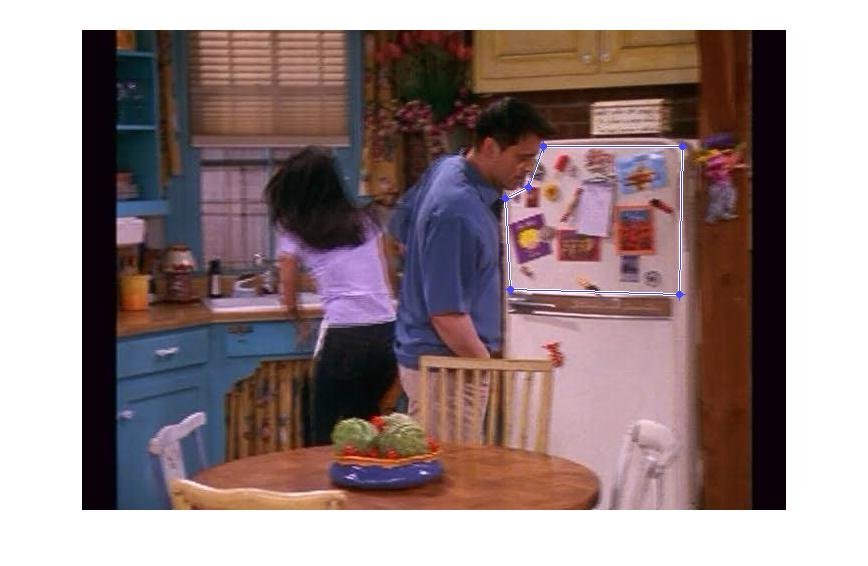
\includegraphics[width = 1\linewidth]{q11.jpg}
\caption{The Polygon I Chose}
\label{q11}
\end{figure}

\begin{figure}
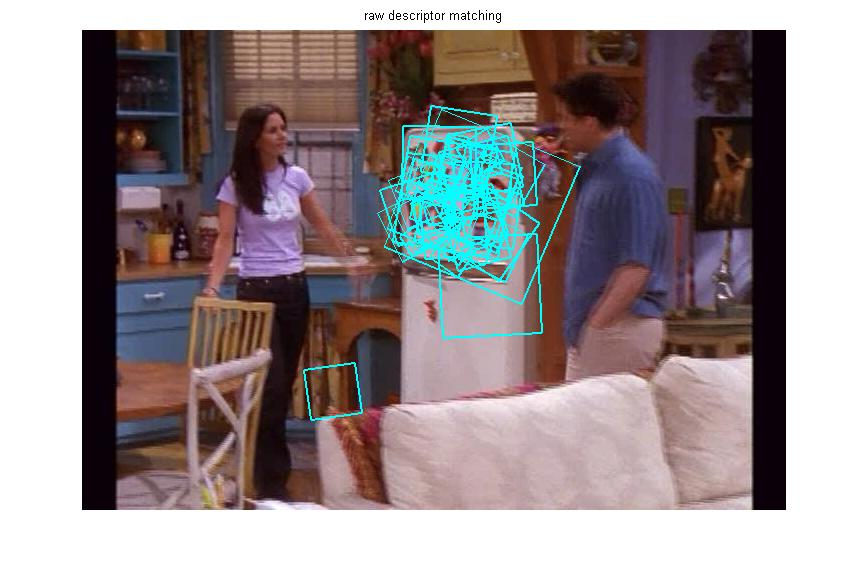
\includegraphics[width = 1\linewidth]{q12.jpg}
\caption{Result of Question 1}
\label{q12}
\end{figure}

\subsection{Visualizing the vocabulary}
See \emph{visualizeVocabulary.m}. As mentioned above, the question 2 runs quite slowly. I used 0.1 fraction of frames to generate visual words. It needs about 1 hour to complete generation. I found most of time costs in kmeans cluster. I cluster visual works by K = 1500. You can modify K and PORTION in 7, 8th line of \emph{visualizeVocabulary.m} to change the fraction of frames or number of clusters you want to use for generating visual words. \\
\\
I chose first two of visual words to show in figure \ref{q2}. The two lines each contains 10 examples of the visual words. It seems like that the first visual word is some line across the image and the second feature is an angle about 90 degrees.
\begin{figure}
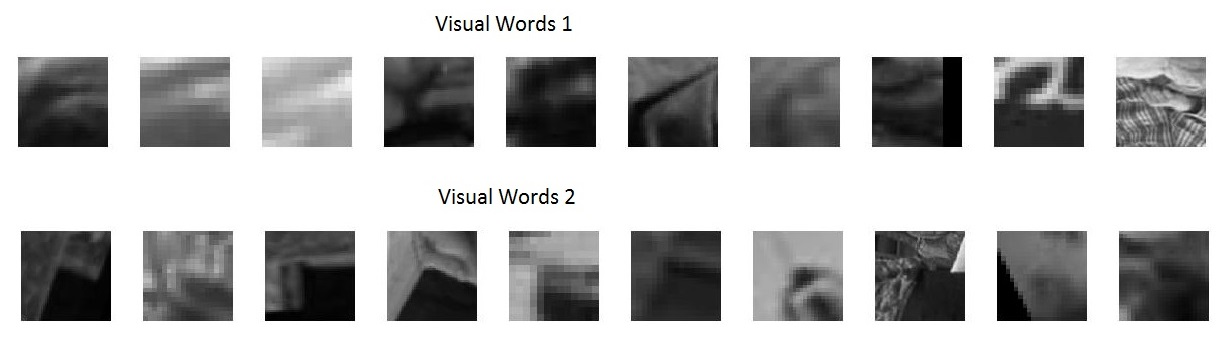
\includegraphics[width = 1.2\linewidth]{q2.jpg}
\caption{Result of Question 1}
\label{q2}
\end{figure}

\subsection{Full frame queries}
See \emph{fullFrameQueries.m}. But this function just call the \emph{regionQueries.m} by set the region to full frame (I implemented this because this two function do almost same thing). So see question 4 for detail explanation of \emph{regionQueries.m}. \\
\\
Two successful (figure \ref{q31}, \ref{q32}) and one fail (figure \ref{q33}) examples:
\begin{figure}
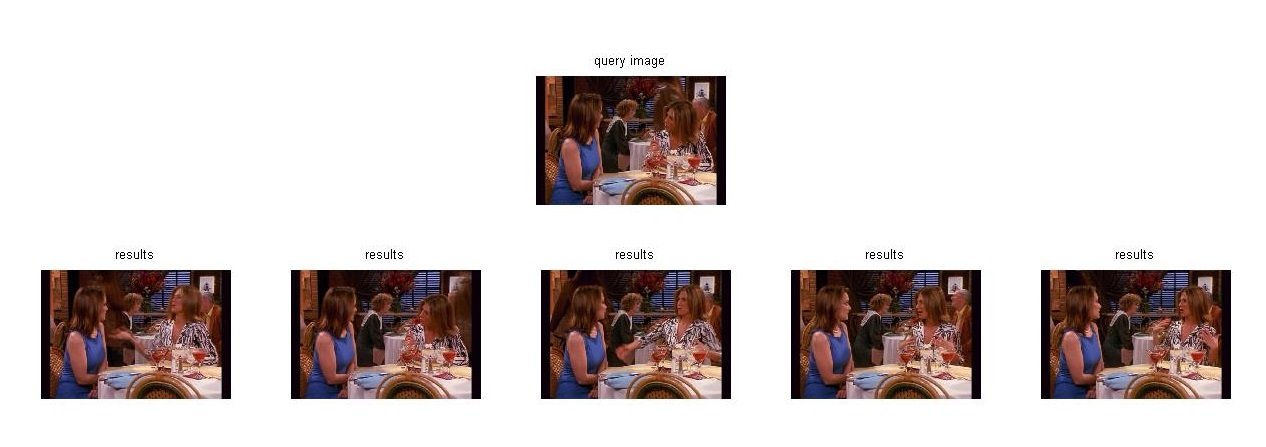
\includegraphics[width = 1.2\linewidth]{q31.jpg}
\caption{Full Frame Query 1}
\label{q31}
\end{figure}

\begin{figure}
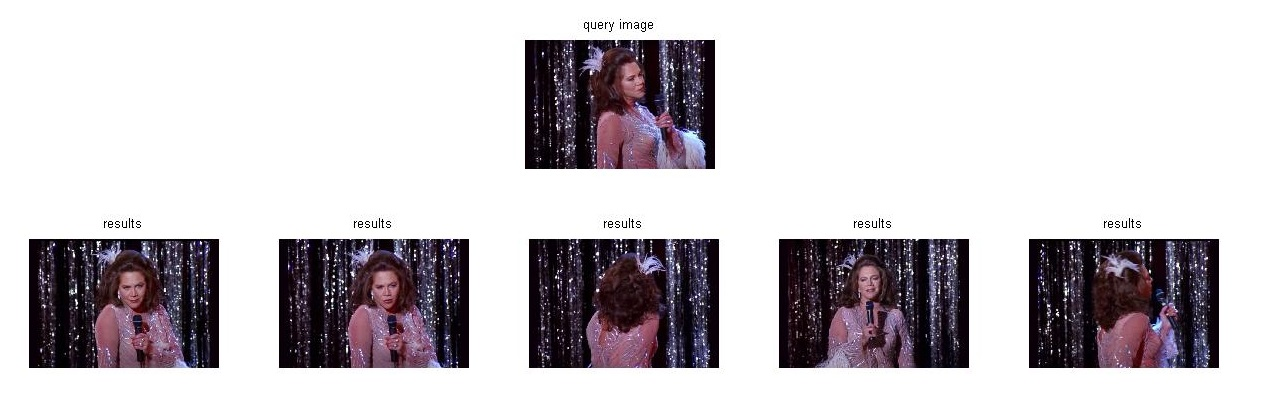
\includegraphics[width = 1.2\linewidth]{q32.jpg}
\caption{Full Frame Query 2}
\label{q32}
\end{figure}

\begin{figure}
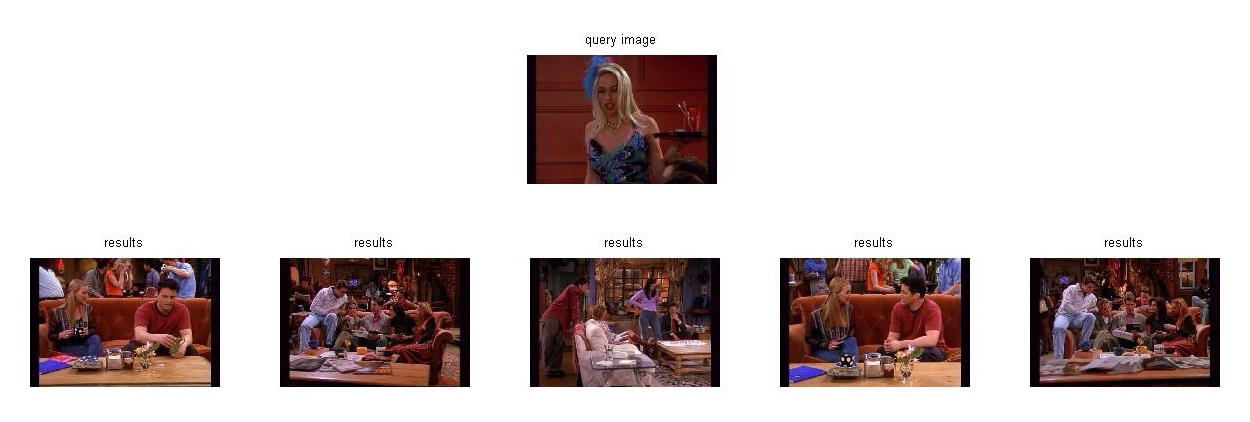
\includegraphics[width = 1.2\linewidth]{q33.jpg}
\caption{Fail Full Frame Query}
\label{q33}
\end{figure}


\subsection{Region queries}
See \emph{regionQueries.m}. This function does bag-of-words matching, using a linear scan through all the ��database�� frames. It matches two frames by comparing two bag-of-words histograms using the normalized scalar product. This function has many optional parameters:
\begin{itemize}
  \item saveToFile, loadFromFile: because compute histograms of all frames cost a lot of time (10 minutes in my experiment). Setting saveToFile true will save the histograms as files in disk. So that you can set loadFromFile true next time you run this function, which makes it outputs result within seconds.
  \item fullFrameQuery: boolean, if true we don't choose region but query full frame
  \item onlyCompareNonZeroWords: boolean, if true, we just count histogram of features in the query region.
  \item useTfidf, ignoreCommon: boolean, if true we will use tfidf, ignore common features. So the extra credit question 1 just set these two true.
\end{itemize}


From results and other experiments I did. I found two kinds of things are easiest to be find in different scenes: 1. woman's cloth with pattern. 2. multiply objects in region. (e.g. bottles on cabinet, stickers on surface of refrigerator). This is because those have many edges, so will have lots of SFIT features, let they be easier to detect in different views. \\

Now I show a woman's cloth detected in other scene (figure \ref{q41}, \ref{q42}) and sticker of refrigerator (figure \ref{q43}, \ref{q44}). Two examples, both can find the region in different scenes.
\begin{figure}
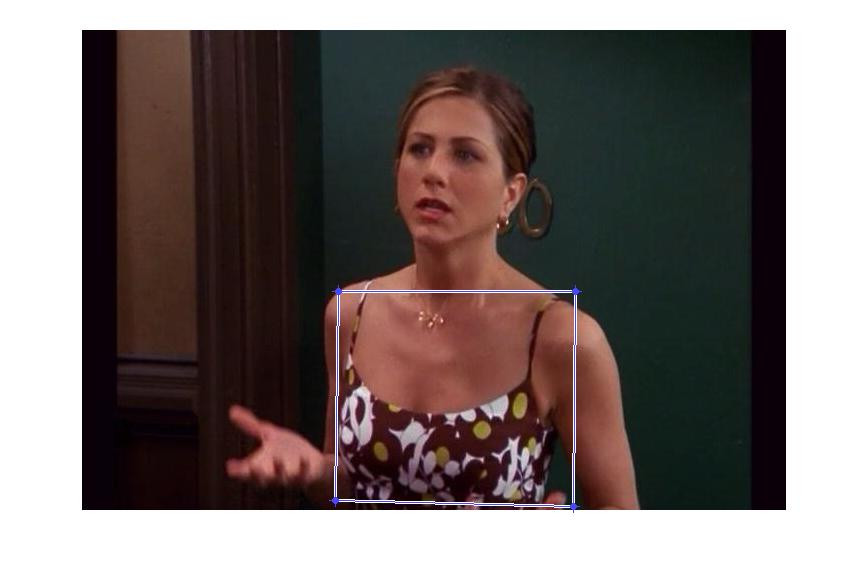
\includegraphics[width = 0.8\linewidth]{q41.jpg}
\caption{Region Query of Woman's Cloth}
\label{q41}
\end{figure}

\begin{figure}
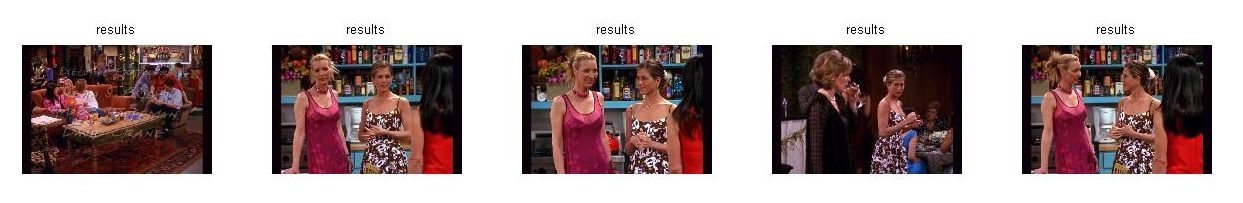
\includegraphics[width = 1.2\linewidth]{q42.jpg}
\caption{Result of Woman's Cloth}
\label{q42}
\end{figure}

\begin{figure}
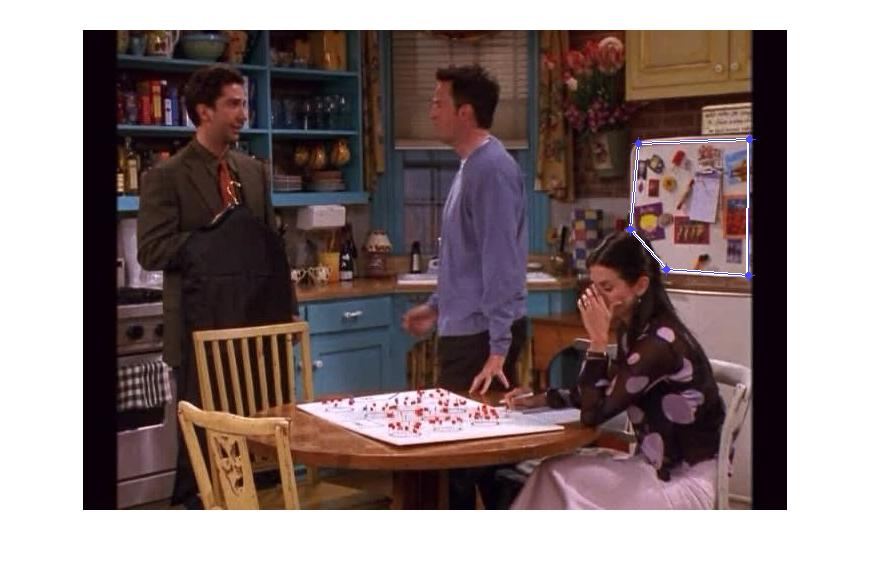
\includegraphics[width = 0.8\linewidth]{q43.jpg}
\caption{Region Query of Stickers}
\label{q43}
\end{figure}

\begin{figure}
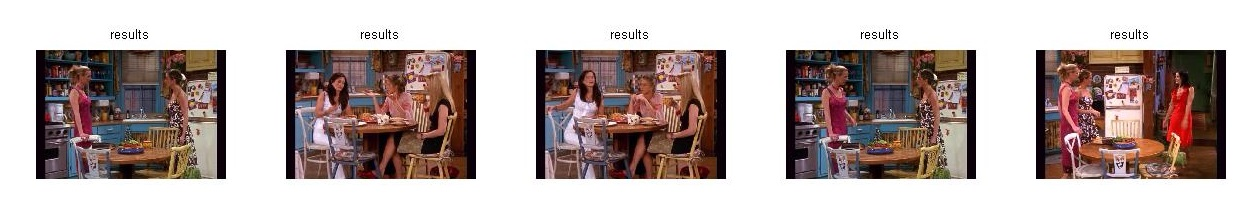
\includegraphics[width = 1.2\linewidth]{q44.jpg}
\caption{Result of Stickers}
\label{q44}
\end{figure}

%\begin{figure}
%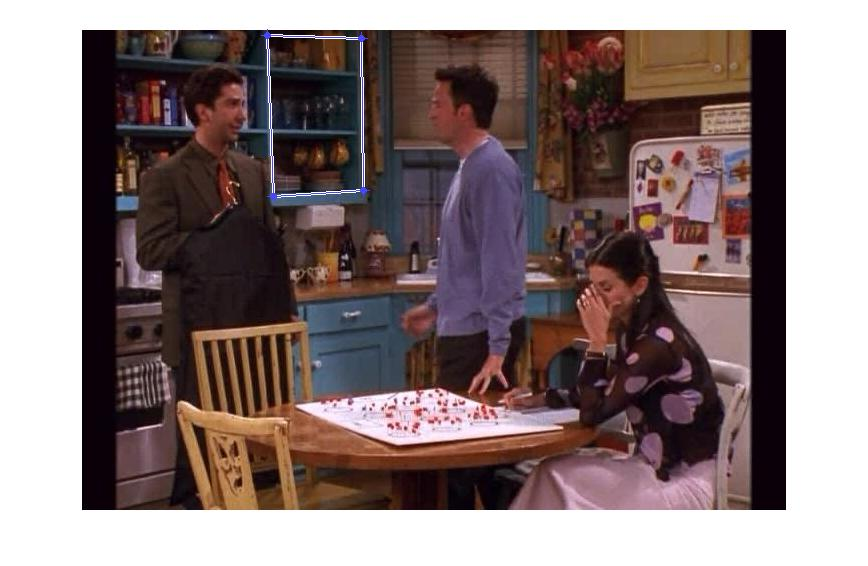
\includegraphics[width = 0.8\linewidth]{q45.jpg}
%\caption{Region Query of Bottles}
%\label{q45}
%\end{figure}

%\begin{figure}
%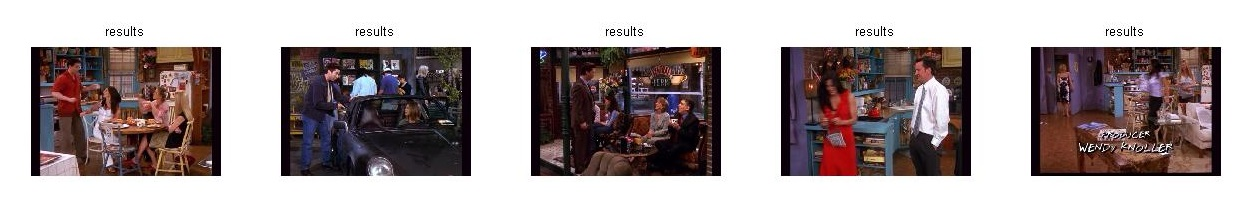
\includegraphics[width = 1.2\linewidth]{q46.jpg}
%\caption{Result of Bottles}
%\label{q46}
%\end{figure}

I found the most common failure case is man's pure color cloth. It doesn't have many edges so few features can be detected. For failure example, figure \ref{q47}, \ref{q48}.
\begin{figure}
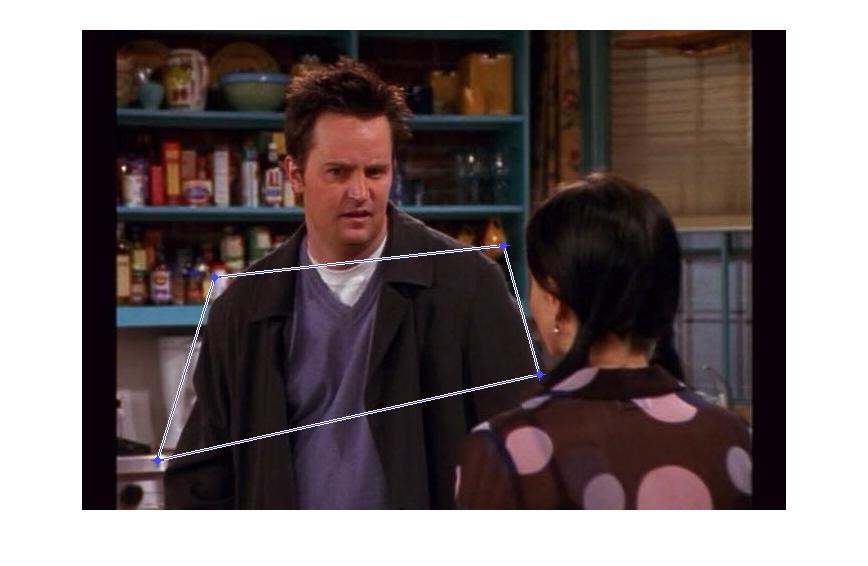
\includegraphics[width = 0.8\linewidth]{q47.jpg}
\caption{Region Query of Man's Cloth}
\label{q47}
\end{figure}

\begin{figure}
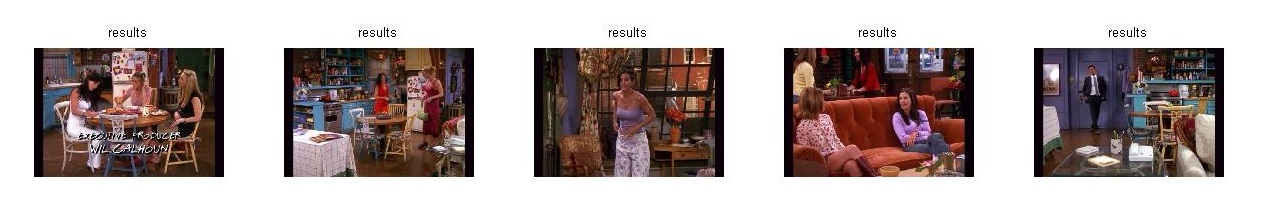
\includegraphics[width = 1.2\linewidth]{q48.jpg}
\caption{Fail Result of Man's Cloth}
\label{q48}
\end{figure}

\section{ Extra Credit }
\subsection{Ignore list and tfidf}
To fun this, just set \textbf{useTfidf, ignoreCommon} parameters of \emph{regionQueries.m} true. How to determine which visual words to be ignore? I counted how many frames the word has occurred. The result was sorted and represented in figure \ref{50}. I ignore those words occurring more than 4000 frames.
\begin{figure}
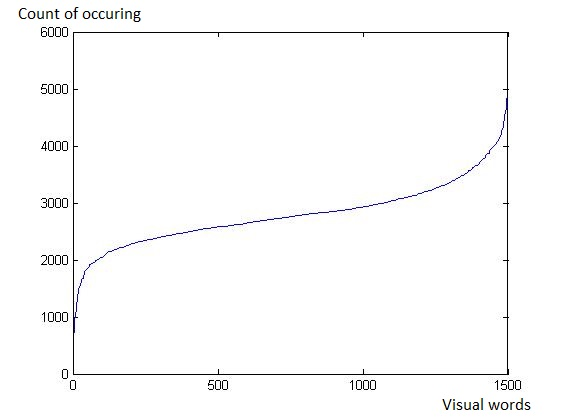
\includegraphics[width = 0.8\linewidth]{50.jpg}
\caption{Sorted Count of Occuring}
\label{50}
\end{figure}

The result improves, I randomly sample 20 frames to compare use/without tfidf and ignoring and check whether the result improves manually (by my eyes). 3 results got better and 1 query got worse. For example, we can see the top 3 rank of using tfidf (figure \ref{51}) is better than those without (figure \ref{52}).
\begin{figure}
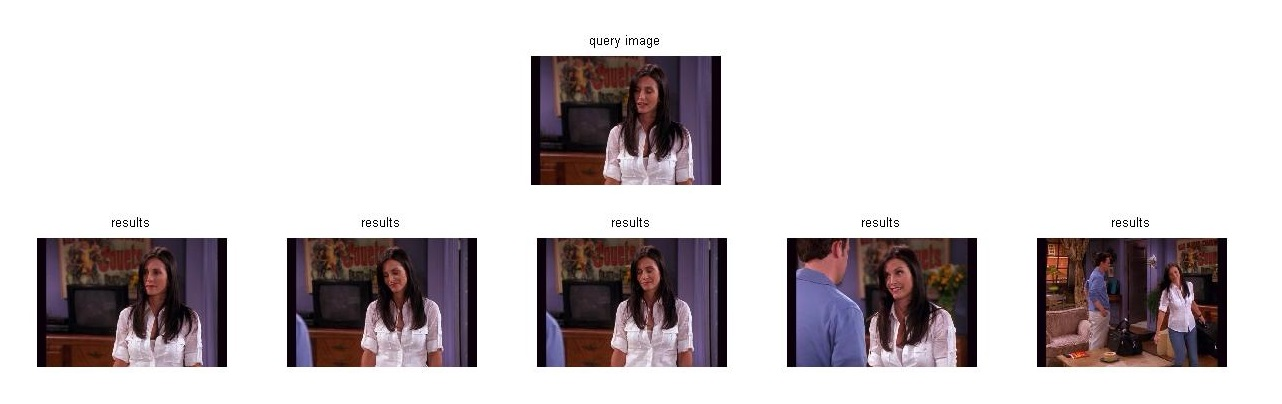
\includegraphics[width = 1.2\linewidth]{51.jpg}
\caption{Result using tfidf and ignoring}
\label{51}
\end{figure}
\begin{figure}
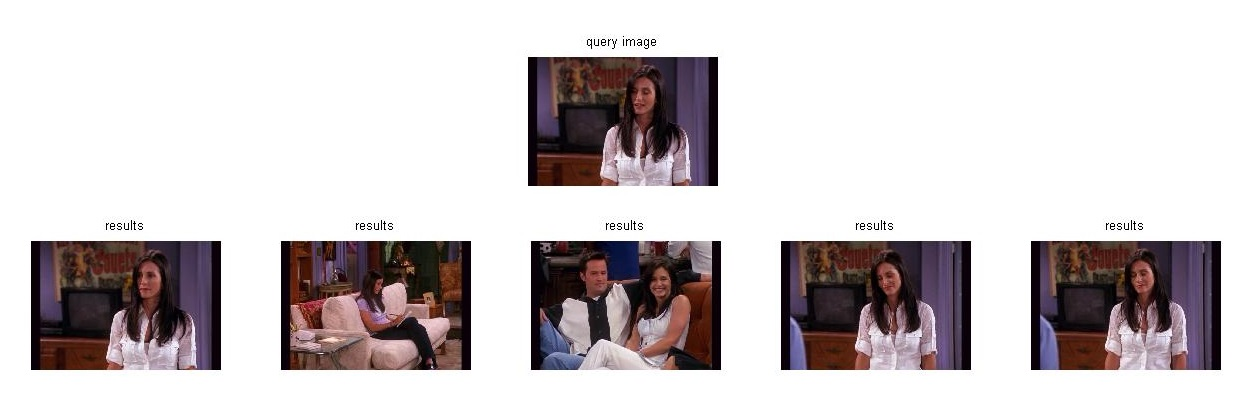
\includegraphics[width = 1.2\linewidth]{52.jpg}
\caption{Result without using tfidf and ignoring}
\label{52}
\end{figure}
\subsection{Shot break detection}
See \emph{shotBreakDetection.m}. I assume that during shot breaking, the bag of words in the scene changes a lot. So I compare histogram of visual words for every adjacent frame pairs by computing normalized Compare two bag-of-words histograms using the
normalized scalar product. Set a threshold. If the normalized scalar product less then the threshold (the two frames show less similarity), then it's a shot break.\\
\\
By setting threshold as 0.2 works well. You can change the threshold at 10th line of \emph{shotBreakDetection.m}. I randomly chose 5 shot break to show in the code, you can see almost every time the 5 pairs of adjacent frames are shot break. See figure \ref{q6}.

\begin{figure}
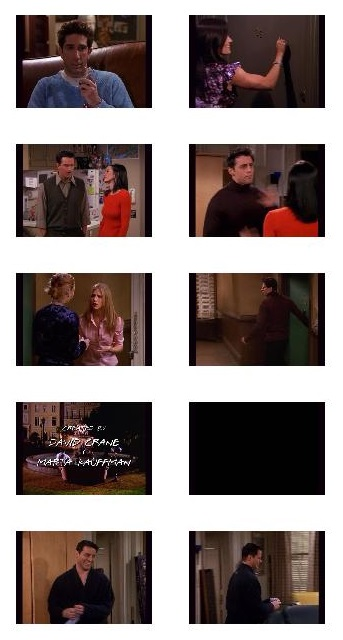
\includegraphics[width = 0.5\linewidth]{q6.jpg}
\caption{Shot Breaks, every row is a pair of two adjacent frames}
\label{q6}
\end{figure}

%\end{CJK*}
\end{document}
